\section{Formal transformation rules}
In this section we will describe how we may transformation a single line of modules in a configuration into other configurations which may be more efficient. In the first section we describe some basic mathematical sets that are used to describe the transformation rules in the following subsections.

\section{Common sets} 
In this section we will try to define a factory configuration using mathematical sets. The sets presented here are used to explain transformation rules in the following subsections.

Previously we presented recipes as acyclic dependency graphs. However at this level of abstraction we do not require the order in which works must be performed. Thus a recipe is simply defined as the set of works needed to be performed on it: 

\[recipe: \textit{A set of all work required to be done by a concrete recipe}\]

A factory configuration is made up of modules. Each module is defined by the following tuple:

\[module: \textit{(aW, mW, up, right, down, left, shadow)}\]

\noindent Where each element of the tuple represents the following:
\begin{itemize}
\item $aW$: The set of work that the module is actively doing.
\item $mW$: The set of work that the module can do.
\item $up,\, right,\, down,\, left$: Describes connections in one of four directions. Each can be either another module or $Ø$.
\item shadow: a boolean indicating whether there is a module placed above or below the module.
\end{itemize}

This definition closely resembles our previous definition of a module. Yet, we add $aW$ as to simplify the logic of our rules. 


In \cref{fig:trivial-example} we see that a configuration is made up of a single line of modules, while \cref{fig:running-example} is made up of three. As such we would like to define a factory configuration as a set of lines of modules, where the flow in each line is moving from left to right.

Let us define a line as a set of modules, which are ordered on the $\prec$ relation. This relation takes two modules $m_1$ and $m_2$ as arguments. It evaluates to true if there is a path from $m_1$ to $m_2$ in the actual factory configuration when we only traverse rightwards. $\prec$ is a total order, and we can thus define a line as a totally ordered set of modules, ordered using $\prec$:

\[line: \textit{A total ordered set of modules ordered on } \prec\]

Having defined recipes, modules and lines we choose to define a factory configuration with the following tuple. 

We now define a configuration as the following tuple:

\[configuration: (R, M, \Gamma)\]

Where:
\[R: \textit{The set of all recipes}\]
\[M: \textit{Set of all modules}\]
\[\Gamma: \textit{The set of all lines}\]


Furthermore we only want each $module$ to appear in a single $line$. To enforce this we set up the following rule for each $line$ $\gamma$, in $\Gamma$:
\[\texttt{if } \gamma \in \Gamma \texttt{ then } \forall m \in \gamma \land \forall \gamma ' \in \Gamma \land \gamma \neq \gamma ',\, m \notin \gamma ' \]


We also set up the following rule for each $module$ $m$ in $M$. This is done to ensure that the module can not perform work not within a recipe, and that the work which it actively performs should be a part of its total set of works:
\[\texttt{if } m \in M \texttt{ then } m.aW \subseteq m.mW \land m.mW \subseteq  \bigcup_{r\in R}r\] 

We also need to describe that not all available modules need to be a part of our factory configuration. There may exist free modules, which are not used, but may aid in the search for a higher throughput. First we describe the set of all modules used by a configuration, denoted $CM$:

\[CM = \{m \in \gamma | \gamma \in \Gamma \}\]

The set of free modules $FM$ is then given by:

\[FM = M \setminus CM \]


\subsection{Anti-serialization}
In \cref{fig:trivial-example} we see that some items will have to move through modules, where no work is performed on them. This will often happen if we have a line of modules, where more than one type of item is to be produced. We would like to describe a rule, which breaks the serial connection of a line of modules. It should be able to make an off branch from a line, moving into the new branch a sequence of modules, which are only used by one type of item. Performing several branches like this across a line, should decrease the amount of unneeded modules which each item need to pass through. This should eventually increase the total throughput.

Let us say that we want to branch out a specific recipe $r$ from a line $\gamma$. Here we first define a special set on $r$, $\bar{r}$, which contains all types of work which are not unique to $r$:
\[\bar{r} = \bigcup_{r' \in R}r', \texttt{ if } r' \neq r\]

Next we need to define what we would like to call common modules. These are module in $\gamma$, which $r$ needs to use along with at least some other recipe. These are important to identify, as they may not be branched out, as that would make the inaccessible to the other recipes that might need it.  Given $r$ and $\gamma$ we define the set of common modules $K_{\gamma ,r}$ as follows:

\[K_{\gamma ,r} = \{m \in \gamma | \gamma \in \Gamma \land \exists \rho \in m.aW,\, \{\rho\} \subseteq r \land \{\rho\} \subseteq \bar{r} \land r \in R\}\]

From this set we can then define $\alpha_{\gamma ,r}$, which is the set of modules in $\gamma$ which are not used by $r$: 

\[\alpha_{\gamma ,r}  = \{m \in \gamma | \gamma \in \Gamma \land \forall \rho \in m.aW,\, \{\rho\} \nsubseteq r \land r \in R\}\]

Along with $\beta_{\gamma ,r}$, which is the set of modules in $\gamma$ used only by $r$:

\[\beta_{\gamma ,r}  = \{m \in \gamma | \gamma \in \Gamma \land \forall \rho \in m.aW,\, \{\rho\} \subseteq r \land \{\rho\} \nsubseteq \bar{r} \land r \in R\}\]

We now want to define a set of all neighbours of common modules in line $\gamma$. Two modules $m_1$ and $m_2$ are said to be neighbours within a set if $m_1 <_k m_2$ holds true. The relation does this if $m_1$ $\prec_r$ $m_2$ evaluates to true, while $m_1$ $\prec_r$ $m_i$ does not hold true for any module in $\gamma$ which is not equal to $m_2$. Having set up this relation, we can define the set of all common module neighbours $KP_{\gamma ,r}$ as:
 
\[KP_{\gamma ,r} = \{(s, e)| {s, e} \in K_{\gamma ,r} \times K_{\gamma ,r} \land s <_k  e\}\]


Let us say that we take a specific pair from $KP_{\gamma ,r}$  known as $(s,e)$. We define the set of all modules in the line $\gamma$ appearing between these two modules as: 

\[M_{s,e} = \{m | m \in \gamma \land \gamma \in \Gamma \land s \prec m \land m \prec e\}\]

We can now define the set of all modules appearing between $s$ and $e$, which are not used to work $r$ $A_{s,e}$ as follows: 

\[A_{s,e} = \{m |m \in M_{s,e} \land m \in \alpha\}\]

Similarly we can define the set $B_{s,e}$, which contains all modules that appear between $s$ and $e$ which are only used to perform work on $r$

\[B_{s,e} = \{m |m \in M_{s,e} \land m \in \beta\}\]

Having now defined our sets, we will set up the rules describing how we may branch out modules to work on individual recipes. These rules will be described informally using our own graphical notation. Imagine we are in the situation stated in 

\begin{figure}[h]
\centering
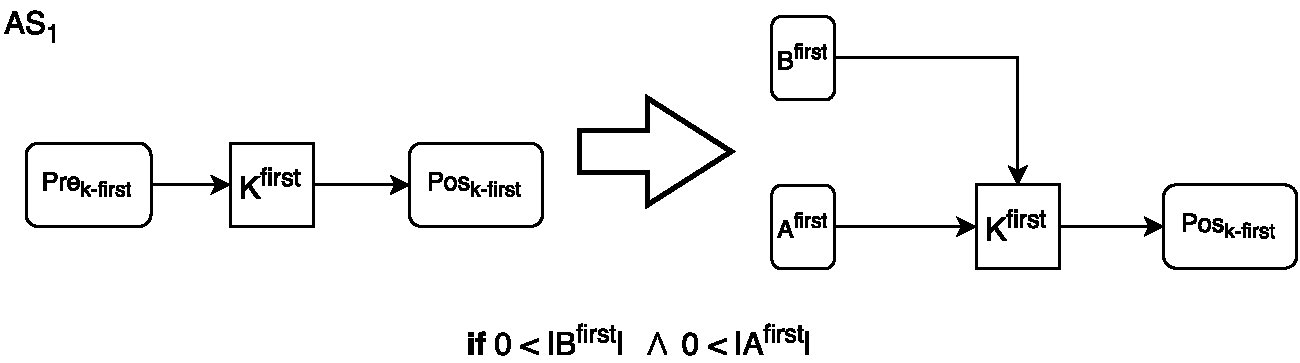
\includegraphics[width=\textwidth]{as1.pdf}
\caption{A trivial configuration of a toy factory layout}
\label{fig:asbase}
\end{figure}


Something about inbranching
\[Pre_{s} = \{m | m \in \gamma \land \gamma \in \Gamma \land m \prec s\}\]

Something about outbranching
\[Post_{e} = \{m | m \in \gamma \land \gamma \in \Gamma \land e \prec  m \}\]



\subsection{Parallel production}

\[Map_{s, e} = \{(m, m')| m \in FM \land m' \in M_{s,e} \land m'.aW \subseteq m.mW\} \]

We define $s[1]$ as the operation that given a set of pairs $s$, gives the set of all the first elements of the pairs in $s$ and $s[2]$ as the operation that gives the second elements.
\[s[1] = \{m_1 | (m_1, m_2) \in s\}\]
\[s[2] = \{m_2 | (m_1, m_2) \in s\}\]

\[MapPaths_{s,e} = \{p \in {Map}_{s,e}^2 | (m,m') \in p \land (n,n') \in p \land |p| = |M_{s,e}| \land  \forall m': m' \neq n' \}\]

\[ PPaths_{s,e} = \{p[1] | p \in MapPaths_{s,e}\}\]

\[a <_{p} b = 
\left\{\begin{matrix}
tt \texttt{ if } x \prec y \land (x, a), (y, b) \in MapPaths_{s,e}])\\
\texttt{else } ff
\end{matrix}\right.\]



\subsection{Swap}

